\documentclass[]{article}
\usepackage{lmodern}
\usepackage{amssymb,amsmath}
\usepackage{ifxetex,ifluatex}
\usepackage{fixltx2e} % provides \textsubscript
\ifnum 0\ifxetex 1\fi\ifluatex 1\fi=0 % if pdftex
  \usepackage[T1]{fontenc}
  \usepackage[utf8]{inputenc}
\else % if luatex or xelatex
  \ifxetex
    \usepackage{mathspec}
  \else
    \usepackage{fontspec}
  \fi
  \defaultfontfeatures{Ligatures=TeX,Scale=MatchLowercase}
\fi
% use upquote if available, for straight quotes in verbatim environments
\IfFileExists{upquote.sty}{\usepackage{upquote}}{}
% use microtype if available
\IfFileExists{microtype.sty}{%
\usepackage{microtype}
\UseMicrotypeSet[protrusion]{basicmath} % disable protrusion for tt fonts
}{}
\usepackage[margin=1in]{geometry}
\usepackage{hyperref}
\hypersetup{unicode=true,
            pdftitle={Kiritimati PPQ Data Exploration},
            pdfauthor={Kevin Bruce, John Burns, Kailey Pascoe, \& Julia Baum},
            pdfborder={0 0 0},
            breaklinks=true}
\urlstyle{same}  % don't use monospace font for urls
\usepackage{graphicx,grffile}
\makeatletter
\def\maxwidth{\ifdim\Gin@nat@width>\linewidth\linewidth\else\Gin@nat@width\fi}
\def\maxheight{\ifdim\Gin@nat@height>\textheight\textheight\else\Gin@nat@height\fi}
\makeatother
% Scale images if necessary, so that they will not overflow the page
% margins by default, and it is still possible to overwrite the defaults
% using explicit options in \includegraphics[width, height, ...]{}
\setkeys{Gin}{width=\maxwidth,height=\maxheight,keepaspectratio}
\IfFileExists{parskip.sty}{%
\usepackage{parskip}
}{% else
\setlength{\parindent}{0pt}
\setlength{\parskip}{6pt plus 2pt minus 1pt}
}
\setlength{\emergencystretch}{3em}  % prevent overfull lines
\providecommand{\tightlist}{%
  \setlength{\itemsep}{0pt}\setlength{\parskip}{0pt}}
\setcounter{secnumdepth}{0}
% Redefines (sub)paragraphs to behave more like sections
\ifx\paragraph\undefined\else
\let\oldparagraph\paragraph
\renewcommand{\paragraph}[1]{\oldparagraph{#1}\mbox{}}
\fi
\ifx\subparagraph\undefined\else
\let\oldsubparagraph\subparagraph
\renewcommand{\subparagraph}[1]{\oldsubparagraph{#1}\mbox{}}
\fi

%%% Use protect on footnotes to avoid problems with footnotes in titles
\let\rmarkdownfootnote\footnote%
\def\footnote{\protect\rmarkdownfootnote}

%%% Change title format to be more compact
\usepackage{titling}

% Create subtitle command for use in maketitle
\providecommand{\subtitle}[1]{
  \posttitle{
    \begin{center}\large#1\end{center}
    }
}

\setlength{\droptitle}{-2em}

  \title{Kiritimati PPQ Data Exploration}
    \pretitle{\vspace{\droptitle}\centering\huge}
  \posttitle{\par}
    \author{Kevin Bruce, John Burns, Kailey Pascoe, \& Julia Baum}
    \preauthor{\centering\large\emph}
  \postauthor{\par}
      \predate{\centering\large\emph}
  \postdate{\par}
    \date{26 February, 2020}


\begin{document}
\maketitle

{
\setcounter{tocdepth}{2}
\tableofcontents
}
\hypertarget{introduction}{%
\subsection{Introduction}\label{introduction}}

Kiritimati Research Project- PPQ rugosity analyses 2015 - 2019

PPQ = Permenant Photoquadrat (4m X 4m)

This document is for the PPQ data collected on Kiritimati to look at
rugosity changes that occur on reefs following a mass mortality event.

The plots below show a view of the data across different spatial and
temporal scales. We will start by looking at the data braodly before
zooming in to specific PPQ fluctuations over time.

It is important to note that Sites 15 and 19 (both within the Very Low
disturbance category) were unable to be sampled in 2019 due to weather,
however Site 37 in Vaskess Bay was accessible and used as a Very Low
site (VL4) along with Site 5 (VL3).

For reference, here is the map of Kiritimati listing the sites that I
plan to use for the manuscript. Sites H1, H2, and L1 haven't been used
in these analyses as there is no Agisoft Model created to compare yet.
(all will be compared to levels post-El Niño).

\begin{center}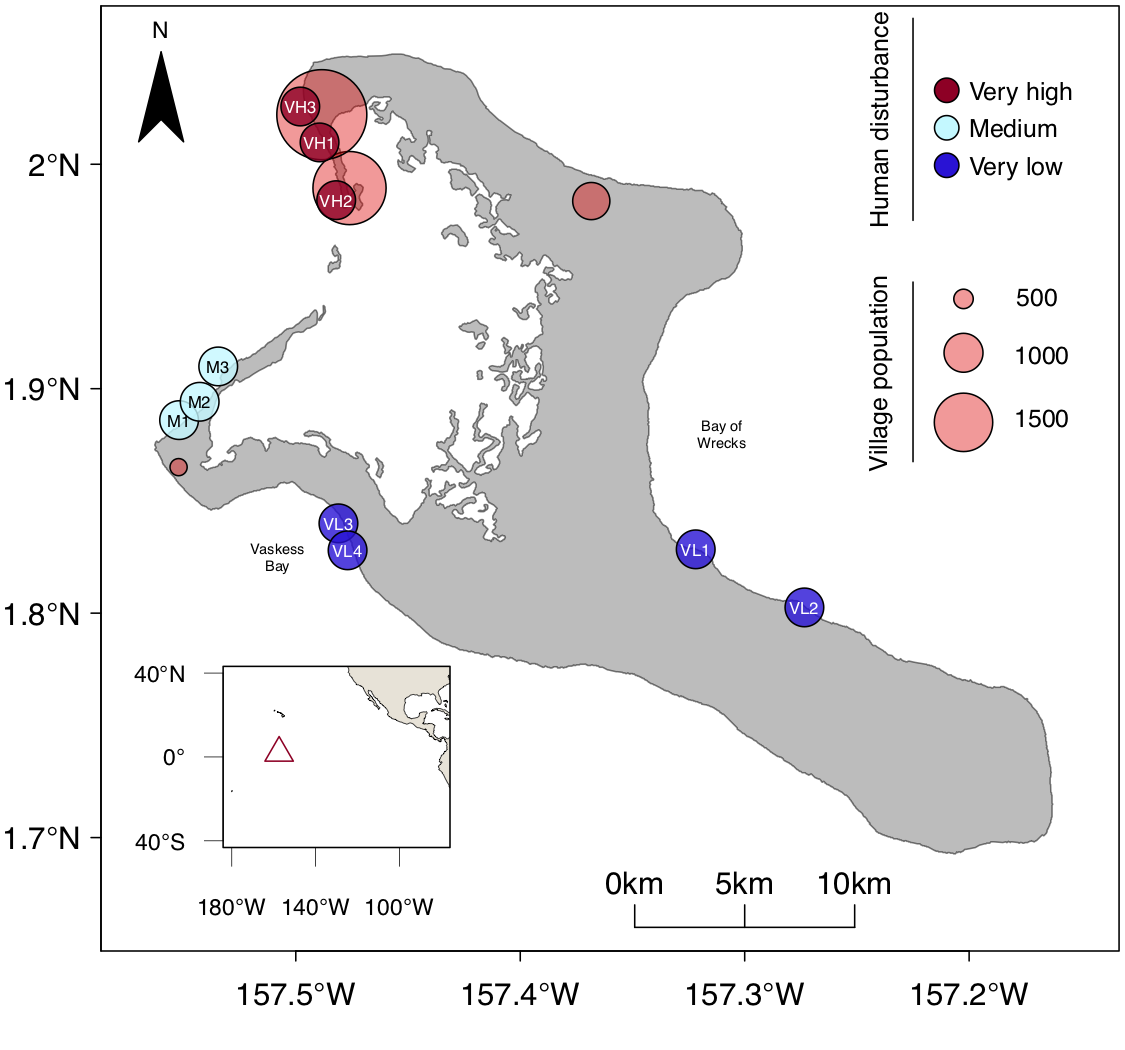
\includegraphics[width=15.62in]{Bruce_MPQ_Analysis_files/figure-latex/map-1} \end{center}

\hypertarget{year-level}{%
\subsection{Year level}\label{year-level}}

The three rugosity metrics are averaged to the year level, showing each
metric's changes across the three time points.

\hypertarget{rugosity}{%
\subsubsection{Rugosity}\label{rugosity}}

\includegraphics{Bruce_MPQ_Analysis_files/figure-latex/Rugosity by year-1.pdf}

There as a large decline between 2015 and 2017, however it appears to
level out when comparing 2017 and 2019.

\hypertarget{terrain-ruggedness}{%
\subsubsection{Terrain Ruggedness}\label{terrain-ruggedness}}

\includegraphics{Bruce_MPQ_Analysis_files/figure-latex/TR/yr-1.pdf}

Similar results that were seen with surface rugosity, to rugosity,
however it seems that Terrain Ruggedness slightly increases from its
lowest point in 2017. Any ideas what could cause that?

\hypertarget{curvature}{%
\subsubsection{Curvature}\label{curvature}}

\includegraphics{Bruce_MPQ_Analysis_files/figure-latex/Abs_curv/yr-1.pdf}

Similar to the previous two plots, curvature appers to stay the same
between 2017 and 2019, although 2019 has the highest variability between
all three sampling periods.

\hypertarget{disturbance-gradient-level}{%
\subsection{Disturbance gradient
level}\label{disturbance-gradient-level}}

The three rugosity metrics are now averaged by disturbance gradient,
which in this case has 3 levels: Very Low, Medium, Very High. These
levels are pre-determined by previous publications taking into effect
the fishing pressure and distance from the human populous.

It's worth noting that the very low sites from 2019 include only 1 that
was sampled in 2015 and 2017, with another that was new that year. We
were unable to get to two of the sites (VL1 and VL2) in 2019 due to
weather.

\hypertarget{rugosity-1}{%
\subsubsection{Rugosity}\label{rugosity-1}}

\includegraphics{Bruce_MPQ_Analysis_files/figure-latex/rug by dist.lvl-1.pdf}

Results show a similar trend to what we witnessed earlier when looking
at the metrics by year, in that 2017 and 2019 values appear relatively
similar, or even with 2019 values slightly increased. The medium sites
appear to be driving the overall increase seen in 2019, with both the
Very Low and Very High sites experiencing similar values to the 2017
value.

\hypertarget{terrain-ruggedness-1}{%
\subsubsection{Terrain Ruggedness}\label{terrain-ruggedness-1}}

\includegraphics{Bruce_MPQ_Analysis_files/figure-latex/TR/hum-1.pdf}

Here we actually see all 3 human disturbance gradients actually
experienced an increase in Terrain ruggedness in 2019 vs 2017. Is it
possible to keep the structure intact and increase TR? TR = grooves and
valleys of the surface, so does this potentially mean that there are
more of these appearing on the reef?

\hypertarget{curvature-1}{%
\subsubsection{Curvature}\label{curvature-1}}

\includegraphics{Bruce_MPQ_Analysis_files/figure-latex/Curv/Human-1.pdf}

Huge variation in the 2019 medium disturabnce gardient, with very high
experiencing expected curvature values. Very low experienced an increase
in curvature values in 2019 to even pre-El nino levels, however site
differences may play a role on this one too.

\hypertarget{site-level}{%
\subsection{Site level}\label{site-level}}

Here I averaged the rugosity metrics by site for each time point
sampled. At this level, declines from 2015 to 2017 were noted as in JM's
paper, but many of the 2019 values seem to increase. Unsure what is
going on?

\hypertarget{rugosity-2}{%
\subsubsection{Rugosity}\label{rugosity-2}}

\includegraphics{Bruce_MPQ_Analysis_files/figure-latex/Rugosity by Site over time-1.pdf}

Some sites are experiencing increases in surface rugosity to levels even
higher than in 2015 (Ex: Site VH2) with many others having larger values
than in 2017 (Ex: VL3, M2). These discrepencies span across the
disturbance gradient as well.

\hypertarget{terrain-ruggedness-2}{%
\subsubsection{Terrain Ruggedness}\label{terrain-ruggedness-2}}

\includegraphics{Bruce_MPQ_Analysis_files/figure-latex/Terrain Ruggedness over time by site-1.pdf}

Same as surface rugosity notes, with site VH2 still having larger TR
values in 2019 than in 2015.

\hypertarget{curvature-2}{%
\subsubsection{Curvature}\label{curvature-2}}

\includegraphics{Bruce_MPQ_Analysis_files/figure-latex/curvature at each site and time period-1.pdf}

Curvature is a bit of an oddball, as a it appears the variation between
sites is huge (very long boxplots), with sites VL3 and M2 having larger
values in 2019 than in 2015. Doesn't seem to be a discernable pattern
here that I can tell.

\hypertarget{ppq-level}{%
\subsection{PPQ level}\label{ppq-level}}

The rugosity metrics are brought down to the PPQ level, with metric
values at each of the three time points the PPQ's were sampled. Sites 15
and 19 were unable to be reached (due to weather) in 2019, hence the two
time points shown.

\hypertarget{rugosity-3}{%
\subsubsection{Rugosity}\label{rugosity-3}}

\includegraphics{Bruce_MPQ_Analysis_files/figure-latex/Each PPQ for each site at each time point-1.pdf}

For a few sites and PPQ's, rugosity has declined, or stayed stable since
2017 {[}as expected{]} but, for some PPQ's and sites, rugosity seems to
increase to 2015 levels or even exceeding them. Eg: Site 32. Not sure
how this could be the case?

\hypertarget{terrain-ruggedness-3}{%
\subsubsection{Terrain Ruggedness}\label{terrain-ruggedness-3}}

\includegraphics{Bruce_MPQ_Analysis_files/figure-latex/TR at each site at each time point-1.pdf}

Similar issue to Rugosity at the PPQ level, some sites are higher in
2019 than in 2017, with site 30 PPQ3 even higher than pre-el Nino in
2015. Site 32 as a whole experienced this, but we are looking at the
orthos for each plot to see if we can visually see a difference
(hypothesis is that this high disturbance sites have lots of loose
abiotic material movement throughout the year)

\hypertarget{curvature-3}{%
\subsubsection{Curvature}\label{curvature-3}}

\includegraphics{Bruce_MPQ_Analysis_files/figure-latex/curvature at each PPQ-1.pdf}

Similar problem, except here its site 35 PPQ 1 \& 2, Site 5 PPQ1 that
have their highest curvature vales in 2019. Why?

\hypertarget{surface-area-of-each-ppq-at-each-time-point}{%
\subsection{Surface Area of each PPQ at each time
point}\label{surface-area-of-each-ppq-at-each-time-point}}

Could the different values we are getting over the 3 time points be
because we are not exactly photographing the same area, despite the
steel stakes being there? Divers did the best they could in ensuring the
location of new, replacement stakes from 2016 onwards were located in
the same area as the intial stake, but given these results, it appears
they weren't as sucessful as hoped.

Values may be slightly off as KB analyzed his plot area from the base of
the metal stakes, whereas JM analyzed her plots from the centre of the
reflectors.

\includegraphics{Bruce_MPQ_Analysis_files/figure-latex/Each PPQs 2D Surface Area at each time point-1.pdf}

In theory, the PPQ's should all be the same (\textasciitilde{}16m2 in
area), however you can see that there is large amounts of variability
between sample time points. This could potentially account for some of
the variability that we are seeing in the previous rugosity
measurements, however I'm not really sure where to go from here. Any
idea how to fix this or experience with this in the past?

\hypertarget{arcmap-output-comparissons}{%
\subsection{ArcMap output
comparissons}\label{arcmap-output-comparissons}}

These plots were done to make sure the differences we were seeing in
rugosity, TR, and cuvature weren't different due to user error. KB
compared the same 3 sites Surface Rugosity and Terrain Ruggedness values
to those reported by JM and found that his values were very similar to
hers. Note: Values may be slightly off as KB analyzed his plot area from
the base of the metal stakes, whereas JM analyzed her plots from the
centre of the reflectors.

\hypertarget{rugosity-4}{%
\subsubsection{Rugosity}\label{rugosity-4}}

\includegraphics{Bruce_MPQ_Analysis_files/figure-latex/Rugosity KB vs. JM-1.pdf}

KB and JM's values are close, however 5.2 (Site5-PPQ2) and 8.3 (Site
8-PPQ3) are off enough that KB should go back and redo JM's metric
calculations from the base of the stakes.

\hypertarget{terrain-ruggedness-4}{%
\subsubsection{Terrain Ruggedness}\label{terrain-ruggedness-4}}

\includegraphics{Bruce_MPQ_Analysis_files/figure-latex/TR KB Vs. JM-1.pdf}

Values appear consistent between processor, however with rugosity being
different, values collected for JM's paper will need to be redone for
this one from the base of the metal stakes, not from the plastic
reflectors.

\hypertarget{curvature-4}{%
\subsubsection{Curvature}\label{curvature-4}}

\includegraphics{Bruce_MPQ_Analysis_files/figure-latex/Curvature values KB Vs. JM-1.pdf}

Similar to rugosity results, where the differences between measurements
are too high to use JM's values from her results. Unsure as to what is
causing these discrepencies. Additionally, while these values align with
similar values to what JM has received, they are not what ArcMAP help
uses to describe Curvature. Is there a way that we can scale these where
we are able to set the range of values to a range used in other
publicized studies, from say -1 to 1?

\hypertarget{plot-2d-surface-area-comparissons}{%
\subsection{Plot 2D Surface Area
Comparissons}\label{plot-2d-surface-area-comparissons}}

While those values are similar, the area of each plot is different
between processors as KB went to the base of the metal stakes and JM
went to the centre of the reflectors, as shown below by the differing
areas of the plots.

\includegraphics{Bruce_MPQ_Analysis_files/figure-latex/Area Measurements-1.pdf}

This plot highlights the differences in plot area that occur based on
where the corners of the plot are digitized in ArcMap. JM's digitized
vertices were located on the reflectors while KB's are at the base of
the metal stakes. In conclusion, KB should redo JM's plots form 2015 and
2017 to have the plot vertices at the base of the metal stakes vs the
reflectors.

\hypertarget{future-work}{%
\subsection{Future work}\label{future-work}}

\begin{enumerate}
\def\labelenumi{\arabic{enumi}.}
\item
  Potentially look at how the planiform and profile curavtures differ
  across time points? I was reading that profile curvature affects the
  acceleration and deceleration fo flow ==\textgreater{} Perhaps higher
  plots experiencing higher values of this will experience faster
  erosion rates?
\item
  At a conference I just attended, a post-doc inquired whether Ocean
  Acidification could play a role on this. Perhaps it is eroding the
  rock and opening up more of those ``nooks and crannies'', thereby
  enabling the TR values to increase?
\end{enumerate}


\end{document}
